%%
%% This is file `sample-sigconf-authordraft.tex',
%% generated with the docstrip utility.
%%
%% The original source files were:
%%
%% samples.dtx  (with options: `all,proceedings,bibtex,authordraft')
%% 
%% IMPORTANT NOTICE:
%% 
%% For the copyright see the source file.
%% 
%% Any modified versions of this file must be renamed
%% with new filenames distinct from sample-sigconf-authordraft.tex.
%% 
%% For distribution of the original source see the terms
%% for copying and modification in the file samples.dtx.
%% 
%% This generated file may be distributed as long as the
%% original source files, as listed above, are part of the
%% same distribution. (The sources need not necessarily be
%% in the same archive or directory.)
%%
%%
%% Commands for TeXCount
%TC:macro \cite [option:text,text]
%TC:macro \citep [option:text,text]
%TC:macro \citet [option:text,text]
%TC:envir table 0 1
%TC:envir table* 0 1
%TC:envir tabular [ignore] word
%TC:envir displaymath 0 word
%TC:envir math 0 word
%TC:envir comment 0 0
%%
%% The first command in your LaTeX source must be the \documentclass
%% command.
%%
%% For submission and review of your manuscript please change the
%% command to \documentclass[manuscript, screen, review]{acmart}.
%%
%% When submitting camera ready or to TAPS, please change the command
%% to \documentclass[sigconf]{acmart} or whichever template is required
%% for your publication.
%%
%%
\documentclass[sigconf,authordraft]{acmart}
%%
%% \BibTeX command to typeset BibTeX logo in the docs
\AtBeginDocument{%
  \providecommand\BibTeX{{%
    Bib\TeX}}}

%% Rights management information.  This information is sent to you
%% when you complete the rights form.  These commands have SAMPLE
%% values in them; it is your responsibility as an author to replace
%% the commands and values with those provided to you when you
%% complete the rights form.
\setcopyright{acmlicensed}
\copyrightyear{2025}
\acmYear{2025}
\acmDOI{XXXXXXX.XXXXXXX}
%% These commands are for a PROCEEDINGS abstract or paper.
\acmConference[GOOD 25 'good25]{GOOD 2025}{March 10--13,
  2025}{Boston, USA}
%%
%%  Uncomment \acmBooktitle if the title of the proceedings is different
%%  from ``Proceedings of ...''!
%%
%%\acmBooktitle{Woodstock '18: ACM Symposium on Neural Gaze Detection,
%%  June 03--05, 2018, Woodstock, NY}
%\acmISBN{978-1-4503-XXXX-X/18/06}


%%
%% Submission ID.
%% Use this when submitting an article to a sponsored event. You'll
%% receive a unique submission ID from the organizers
%% of the event, and this ID should be used as the parameter to this command.
%%\acmSubmissionID{123-A56-BU3}

%%
%% For managing citations, it is recommended to use bibliography
%% files in BibTeX format.
%%
%% You can then either use BibTeX with the ACM-Reference-Format style,
%% or BibLaTeX with the acmnumeric or acmauthoryear sytles, that include
%% support for advanced citation of software artefact from the
%% biblatex-software package, also separately available on CTAN.
%%
%% Look at the sample-*-biblatex.tex files for templates showcasing
%% the biblatex styles.
%%

%%
%% The majority of ACM publications use numbered citations and
%% references.  The command \citestyle{authoryear} switches to the
%% "author year" style.
%%
%% If you are preparing content for an event
%% sponsored by ACM SIGGRAPH, you must use the "author year" style of
%% citations and references.
%% Uncommenting
%% the next command will enable that style.
%%\citestyle{acmauthoryear}

\usepackage{tikz}
\usepackage{fontawesome5}
\usetikzlibrary{shapes.geometric, shapes.symbols, arrows, positioning, fit, backgrounds}
%%
%% end of the preamble, start of the body of the document source.
\begin{document}

%%
%% The "title" command has an optional parameter,
%% allowing the author to define a "short title" to be used in page headers.
\title{Securely exposing web services on Open OnDemand}

%%
%% The "author" command and its associated commands are used to define
%% the authors and their affiliations.
%% Of note is the shared affiliation of the first two authors, and the
%% "authornote" and "authornotemark" commands
%% used to denote shared contribution to the research.
\author{Harry Smallbone}
\orcid{0009-0004-3865-5624}
\affiliation{%
  \institution{University of Western Australia}
  \country{}
}
\email{harry.smallbone@research.uwa.edu.au}

\author{Thomas Drake-Brockman}
\orcid{0000-0002-7649-3951}
\affiliation{%
  \institution{University of Western Australia}
  \country{}
  }
\email{thomas.drake-brockman@uwa.edu.au}

\author{Britta von Ungern-Sternberg}
\orcid{0000-0002-8043-8541}
\affiliation{%
  \institution{University of Western Australia}
  \country{}
}
\email{britta.regli-vonungern@uwa.edu.au}

%%
%% By default, the full list of authors will be used in the page
%% headers. Often, this list is too long, and will overlap
%% other information printed in the page headers. This command allows
%% the author to define a more concise list
%% of authors' names for this purpose.
%% \renewcommand{\shortauthors}{Smallbone et al.}

%%
%% The abstract is a short summary of the work to be presented in the
%% article.
\begin{abstract}
  Our multidisciplinary team of medical researchers, software engineers, and data analysts deployed a trusted research environment using Open OnDemand inside Perth Children's Hospital to facilitate high performance computing on sensitive healthcare data. We developed an extension to Open OnDemand using Podman to enhance security and allow for user apps to securely expose web services to hospital users. This allows modern web applications to be deployed as-is using their standard deployment workflow, typically Dockerfile or Kubernetes based. The deployed extension is in use for multiple applications on healthcare data at Perth Children's Hospital.
\end{abstract}

%%
%% Keywords. The author(s) should pick words that accurately describe
%% the work being presented. Separate the keywords with commas.
\keywords{HPC, containers, security}
%% A "teaser" image appears between the author and affiliation
%% information and the body of the document, and typically spans the
%% page.
%\begin{teaserfigure}
% \includegraphics[width=\textwidth]{sampleteaser}
%  \caption{Seattle Mariners at Spring Training, 2010.}
%  \Description{Enjoying the baseball game from the third-base
%  seats. Ichiro Suzuki preparing to bat.}
%  \label{fig:teaser}
%\end{teaserfigure}

\received{26 September 2025}

%%
%% This command processes the author and affiliation and title
%% information and builds the first part of the formatted document.
\maketitle

\section{Introduction}
Open OnDemand \cite{Hudak2018} is a web framework for high performance computing (HPC) users to access and run a variety of customisable HPC applications in a web context, frequently including code-focused applications such as R Studio, Jupyter Lab, VS Code Server, and also SSH and remote desktop access. From a system architecture perspective \cite{OODArch} this involves a coordinating web server namely Apache httpd which communicates and submits jobs to a queuing system via a user-level nginx server running Passenger. Security considerations such as authentication and authorisation are user-configurable via Apache configuration or at the application level in Bash scripts. This leads to significant diversity in approaches to security and often leads to hidden dependencies on host and OS security considerations such as SELinux, network namespaces and filesystem permissions. After customisation, Open OnDemand is a powerful tool to access HPC resources remotely. 


The Paediatric Anaesthesia Research Team, part of the Institute for Paediatric Perioperative Excellence (IPPE) at the University of Western Australia, develops and implements clinical research in perioperative anaesthesia according to consumer priorities \cite{blind_sommerfield_consumer_2023} including safer anaesthesia for kids, reducing perioperative anxiety and improving care for patients from regional and remote Australia. Our team consists of multidisciplinary researchers including clinicians, software engineers, data analysts and research assistants. In 2024 we received a grant from the Stan Perron Charitable Foundation to deploy a small on-premises HPC system called MERLIN to allow a diverse range of users from less-technical to highly technical to run local artificial intelligence (AI) on sensitive healthcare data. Our design requirements called for a system that was secure, interoperated with internal enterprise authentication and authorisation, allowed for sharing of limited compute resources and was accessible to our less technical users. We chose Open OnDemand as the primary mode of access to MERLIN. 

The primary use case of our cluster is to design and deploy AI applications in a web context. The most straightforward way to host these applications is as Open OnDemand applications which will be run in a secure self-contained environment in the user context with access to the relevant data. However, there are a number of challenges to doing this natively in Open OnDemand. Accordingly we designed and built a software service called MERLIN OnDemand Proxy to simplify these bespoke deployments. 

\section{Prior Work}
Trusted research environments have been described by the Australian Research Data Commons (ARDC) as highly secure computing environments that provide remote access to sensitive data for analysis and research \cite{ward_trusted_2024}. The Australian government recommends the use of the Five Safes approach developed in the United Kingdom when working with sensitive data for research; Safe People, Safe Projects, Safe Data, Safe Settings and Safe Outputs. TREs lie within the Safe Settings part of this framework. 

According to the Five Safes framework, TREs should be designed to allow external researchers to access sensitive data that has been deidentified in a secure trusted way. This is the approach taken by other extant TREs in Australia such as QCIF KeyPoint, Secure Unified Research Environment (SURE), UNSW ERICA, Monash Secure Research Platform (SeRP) and Curtin SeRP which provide encrypted access to Windows virtual desktop instances with access to deidentified sensitive datasets. The NHS Secure Data Environment Service also follows this approach by providing a secure Databricks instance for researchers to interact with pseudonymised datasets. This allows researchers to both securely access data within a restricted environment and transfer deidentified data outside of the hospital network environment into an external TRE hosted at a research institution.

Outside of the Five Safes framework, TREs vary considerably in scope and design. One example is Finland's CSC - IT Center for Science service ePouta, which facilitates deployments of virtual machines (VMs) and storage resources directly into target institutions using encrypted containerised virtual environment software stacks \cite{noauthor_sensitive_nodate}. Another example is Sweden's Bianca HPC system hosted at Uppsala University, which creates a virtualised cluster with isolated storage and network volumes per project to avoid inter-project contamination \cite{noauthor_bianca_2024}.

\section{Design}
The MERLIN cluster was co-designed with our enterprise security team according to the Five Safes framework. We used Red Hat Enterprise Linux as the OS with SELinux enabled, Slurm for job scheduling, rootless Podman as well as Apptainer for container support and Microsoft Entra ID for network authorisation. Due to corporate network restrictions, we host Open OnDemand from one domain and disallow subdomains.

\begin{figure*}[t!]
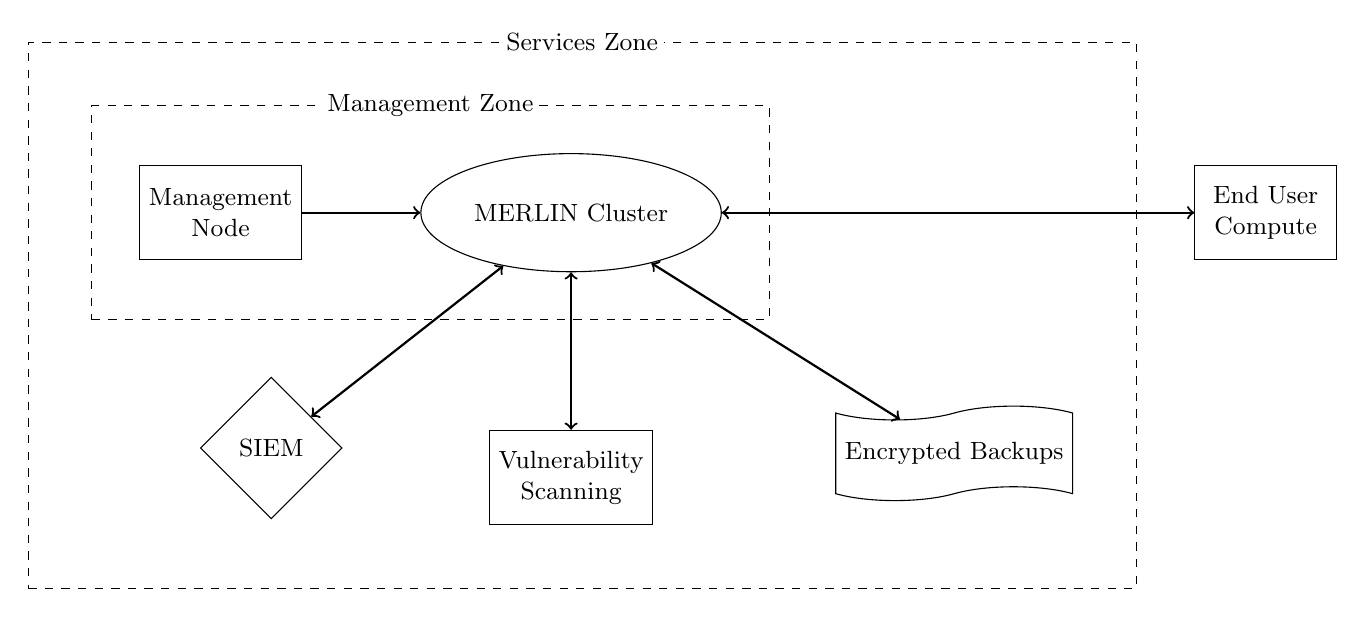
\begin{tikzpicture}[
    box/.style={draw, rectangle, minimum width=1.8cm, minimum height=1.2cm, align=center, font=\small},
    label/.style={font=\small\itshape},
    zone_label/.style={font=\small, fill=white, inner sep=2pt},
    central/.style={draw, ellipse, minimum width=2.2cm, minimum height=1.5cm, align=center, font=\small},
    siem/.style={draw, diamond, minimum width=1.8cm, minimum height=1.8cm, align=center, font=\small},
    backup/.style={draw, tape, minimum width=1.8cm, minimum height=1.2cm, align=center, font=\small}
]

% Central computer
\node[central] (central) {MERLIN Cluster};

% Admin management computer
\node[box, left=1.5cm of central] (admin) {Management\\Node};

% Zone 0 firewall (Management Zone)
\node[fit=(central)(admin), draw, dashed, inner sep=0.6cm] (zone0) {};
\node[zone_label] at (zone0.north) {Management Zone};

% Boxes in Zone 1
\node[siem, below left=2cm and 2cm of central] (siem) {SIEM};
\node[box, below=2cm of central] (vuln) {Vulnerability\\Scanning};
\node[backup, below right=2cm and 2cm of central] (backup) {Encrypted Backups};

% Zone 1 firewall (Services Zone)
\node[fit=(zone0)(siem)(vuln)(backup), draw, dashed, inner sep=0.8cm] (zone1) {};
\node[zone_label] at (zone1.north) {Services Zone};

% End user compute (outside zones)
\node[box, right=6cm of central.east] (enduser) {End User\\Compute};

% SSH connection
\draw[->, thick] (admin) -- (central);

% Bidirectional arrow to end user compute
\draw[<->, thick] (central) -- (enduser);

% Bidirectional connections to services
\draw[<->, thick] (central) -- (siem);
\draw[<->, thick] (central) -- (vuln);
\draw[<->, thick] (central) -- (backup);

\end{tikzpicture}
\caption{Logical network layout}
\end{figure*}

We identified the following common requirements for modern web services.
\begin{enumerate}
    \item An Open Container Initiative (OCI)-compatible container service
    \item Isolation of internal and external network services such that internal databases and services are not externally accessible
    \item Authorisation and authentication
    \item Root domain routing - hosting applications under a URL sub path is frequently not supported
\end{enumerate}
The default Open OnDemand architecture \cite{OODArch} leaves these requirements out of its design and up to user specification. The most commonly suggested solution is to use Open OnDemand's built-in reverse proxy, which routes requests via a sub-path \url{/rnode/<host>/<port>/<application-specific-path>}, along with an additional authorisation server such as Python's Twisted package. However, this configuration requires the application to support sub-path URL rewriting and leaves open the possibility of brute-forcing ports to gain access to internal services and is therefore not suitable for our use-case. Another possibility may have been to host web services on automatically generated subdomains that are only accessible to users while a job is being run, however due to enterprise network limitations we were unable to access dynamic subdomain generation.

\section{Solution}
We created a defense-in-depth solution to this problem.

Firstly, we separated internal and external network service boundaries by creating a common Open OnDemand containerised design that enforces a single entry point Caddy web server. We additionally used the OOD Proxy project from Brigham Young University \cite{noauthor_byuhpcoodproxy_2025} to generate a per-job Linux network namespace to further isolate users from external access. The same approach can be trivially extended to a Kubernetes Pod.

We use the Slurm dependency munge to generate authorisation tokens for individual user jobs. These are stored in the user browser cookies as a compromise between frequent re-authentication and job security. At runtime, the Caddy server verifies that the user supplies a correct and current authorisation token for the given job.

To solve the stateful problem of root domain routing, we created a custom Caddy module that allows Slurm jobs to register their application host and port combinations on the Open OnDemand controller host at job creation time. At runtime, the user is routed to the correct application on the root domain using their authorisation cookie. The Caddy module verifies that user is authenticated, the Slurm job is still running and the validity of the munge token before reverse proxying to the job host.

The final system design is illustrated in Figure 2.

\begin{figure}[H]
% Define styles for the nodes
\tikzstyle{process} = [rectangle, draw=blue, thick, minimum width=3cm, minimum height=1cm, text centered, rounded corners]
\tikzstyle{container} = [rectangle, draw=orange, thick, minimum width=3cm, minimum height=1cm, text centered, rounded corners]
\tikzstyle{dashedline} = [dashed, thick, red]
\tikzstyle{bidirectional} = [<->, thick]
 
\begin{tikzpicture}[node distance=2cm, font=\sffamily]


% Firewall dashed line for column 1
%\draw[dashedline] ([xshift=-2cm]data.south) -- ([xshift=2cm]data.south) node[midway, below] {Firewall};


% Column 2: Researcher to Compute Environment
\node (researcher)  {\faStethoscope \ Researcher};
\node (ood) [process, below of=researcher] {Open OnDemand Web Portal};
\node (cc) [process, below of=ood] {Caddy Reverse Proxy};
\node (proxy) [process, below of=cc] {Open OnDemand Reverse Proxy};
\node (caddy) [container, below of=proxy] {Caddy Server};
\node (compute) [process, below of=caddy, yshift=-0.25cm] {Compute Environment};

% Column 1: Data flow to Computer Storage
\node (data) [above left=-1.4cm and 2.5cm of compute, outer sep=0] {
    \begin{tabular}{c}
        \faFile \ Documents \\[0.2cm]
        \faVolumeUp \ Audio \\[0.2cm]
        \faVideo \ Video
    \end{tabular}
};
\node (eds) [draw=purple, thick, dashed, fit=(data), inner sep=0.25cm] {};
\node[anchor=south west, purple] at (eds.north west) {Hospital Data Store}; 

% Box around Caddy Container and Compute Environment
\node (podman) [draw=purple, thick, dashed, fit=(caddy) (compute), inner sep=0.5cm] {};

% Label for the box (outside, top-left)
\node[anchor=south west, purple] at (podman.north west) {Rootless Podman Network};

% Firewall dashed line for column 2
\draw[dashedline] ([xshift=-2cm]researcher.south) -- ([xshift=2cm]researcher.south) node[midway, below, xshift=-0.8cm] {Firewall};

% Bidirectional arrows for column 2
\draw[bidirectional] (researcher.south) -- (ood.north);
\draw[->, thick] (ood.south) -- (cc); 
\draw[->, thick] (cc) -- (proxy); 
\draw[->, thick] (proxy) -- (caddy);
\draw[->, thick] (caddy) -- (compute);

% Connection from computer storage to compute environment
\draw[->, thick, dashed] (eds.east) -- (compute.west) node[midway, below] {Encrypted Data};

\end{tikzpicture}
\caption{MERLIN OnDemand Proxy workflow}
\end{figure}

\section{Discussion}
The presented proxy workflow has enabled easy deployments of web applications in a trusted hospital environment. The Paediatric Anaesthesia Research Team has commenced translational studies including using LLM services like Open WebUI to convert unstructured data from the digital medical record in Perth Children's Hospital into structured data for risk prediction in paediatric anaesthesia. The use of the proxy means that web applications can be introduced by the technical team that are secure, verifiable and self-contained.

The most prominent limitation currently is the maintenance burden and overhead of using a custom authorisation solution. We have endeavoured to keep the design as simple and flexible as possible however it does introduce complexity in deploying another service on top of Open OnDemand. Future work could include streamlining this complexity within Open OnDemand.

\section{Conclusion}
This paper presents the design and deployment of a configurable proxy for Open OnDemand to support modern web applications. The launched environment provides a secure platform for medical research using modern computational techniques such as LLMs, containerisation and defense in depth.

%%
%% The acknowledgments section is defined using the "acks" environment
%% (and NOT an unnumbered section). This ensures the proper
%% identification of the section in the article metadata, and the
%% consistent spelling of the heading.
\begin{acks}
This research was undertaken with funding and support from Stan Perron Charitable Foundation, the  Child and Adolescent Health Service in Western Australia and The University of Western Australia.
\end{acks}

%%
%% The next two lines define the bibliography style to be used, and
%% the bibliography file.
\bibliographystyle{ACM-Reference-Format}
\bibliography{bib}

\iffalse
\section{Tables}

\begin{table}
  \caption{Frequency of Special Characters}
  \label{tab:freq}
  \begin{tabular}{ccl}
    \toprule
    Non-English or Math&Frequency&Comments\\
    \midrule
    \O & 1 in 1,000& For Swedish names\\
    $\pi$ & 1 in 5& Common in math\\
    \$ & 4 in 5 & Used in business\\
    $\Psi^2_1$ & 1 in 40,000& Unexplained usage\\
  \bottomrule
\end{tabular}
\end{table}

\begin{table*}
  \caption{Some Typical Commands}
  \label{tab:commands}
  \begin{tabular}{ccl}
    \toprule
    Command &A Number & Comments\\
    \midrule
    \texttt{{\char'134}author} & 100& Author \\
    \texttt{{\char'134}table}& 300 & For tables\\
    \texttt{{\char'134}table*}& 400& For wider tables\\
    \bottomrule
  \end{tabular}
\end{table*}

\section{Discussion}
\section{Conclusions}
\begin{figure}[h]
  \centering
  \includegraphics[width=\linewidth]{sample-franklin}
  \caption{1907 Franklin Model D roadster. Photograph by Harris \&
    Ewing, Inc. [Public domain], via Wikimedia
    Commons. (\url{https://goo.gl/VLCRBB}).}
  \Description{A woman and a girl in white dresses sit in an open car.}
\end{figure}
\fi

\end{document}
\endinput